\documentclass{beamer}

%% Pacotes
\usepackage[utf8]{inputenc}              %%Formatação de acentos
\usepackage{xcolor}                      %%Definição de cores
\usepackage[framemethod=tikz]{mdframed} %%Estilização dos slides
\usepackage{tcolorbox}                   %%Mudar ambientes de blocos

%\tcbset{colback=red!5!white,
%colframe=red!75!black,fonttitle=\bfseries} %% Borda das caixas

\usepackage[activate={true,nocompatibility},final,tracking=true,kerning=true,spacing=true,factor=1100,stretch=10,shrink=10,expansion]{microtype}
%% Melhorar caligrafia

\SetTracking{encoding={*}, shape=sc}{0} %Caligrafia de small capitals (smallcaps)


\usepackage{pifont} %Dingbats (simbolos do itemize)


%%%%%% NÃO FUNCIONA PRA CLASSE BEAMER %%%%% ~~~
% \renewcommand\labelitemi{\ding{166}} %definindo o símbolo itemize
% padrão a ser utilizado
% \renewcommand{\item}{\ding{166}}
%\newcommand{\itemm}{\ding{\166}}
% \renewcommand\labelitemi{\ding{52}}
%%%%%%%%%%%%%%%%%%%%%%%%%%%%%%%%%%% ~~~

%% Plano de Fundo, imagem logo-usp.
\usebackgroundtemplate{
  
\includegraphics[width=\paperwidth,
  height=\paperheight]{../Imagens/fundo1.jpg}
}

%% Tema da apresentação
\usetheme{Madrid}
\usecolortheme{seahorse}


\mode<presentation>


\title[Introdução ao \LaTeX]{\Huge{Introdução ao \LaTeX}}

\author[Branquinho]{Pedro Gomes Branquinho \\
  \text{\scriptsize{pedro.branquinho@usp.br}}}

\date[EEL-USP]{\scriptsize{Mini-curso de \LaTeX} \\ Universidade de São Paulo - DEMAR}



%%%%%% ~~~~~~~~~ %%%%%%%%

%%%%%%%%%%% Começo do Corpo do Documento %%%%%%%%%%%%%%%%

%%%%%% ~~~~~~~~~ %%%%%%%%


\begin{document}

%% Imagem de fundo para a apresentação,
{\usebackgroundtemplate{
\includegraphics[width=\paperwidth]{../Imagens/TP.jpg}}

%% Alterar o diretório ''../Imagens/TP.jpg'' para mudar de imagem


%%%%%% Primeira slide, utilizando as variáveis author, date etc.
  \begin{frame}
    \titlepage
  \end{frame}
}


\begin{frame}
  \section{Motivações}
  \frametitle{Motivações}

  \begin{enumerate}
  \item{Programação Unificada}
  \item{Flexibilidade Computacional}
  \item{Open Source}
  \item{Estruturas Reutilizáveis -- Bottom-up}
  \item{Fácil Compartilhamento}
  \end{enumerate}

\end{frame}

\begin{frame}
  \frametitle{Motivações}

  \begin{enumerate}
  \item<1->{Programação Unificada}
  \item<5->{Flexibilidade Computacional}
  \item<2->{Open Source}
  \item<3->{Estruturas Reutilizáveis -- Bottom-up}
  \item<4->{Fácil Compartilhamento}
  \end{enumerate}

\end{frame}

\begin{frame}
  \frametitle{Motivações}

  \begin{enumerate}
  \item<1->[\ding{98}]{Programação Unificada}
  \item<5->[\ding{168}]{Flexibilidade Computacional}
  \item<2->[\ding{170}]{Open Source}
  \item<3->[\ding{171}]{Estruturas Reutilizáveis -- Bottom-up}
  \item<4->[\ding{169}]{Fácil Compartilhamento}
  \end{enumerate}

\end{frame}


\begin{frame}
  \frametitle{Motivações}

  \begin{enumerate}
  \item<1->[{\textcolor{yellow!90!black}{\ding{98}}}]{Programação Unificada}
  \item<5->[\ding{168}]{Flexibilidade Computacional}
  \item<2->[{\textcolor{red}{\ding{170}}}]{Open Source}
  \item<3->[\ding{171}]{Estruturas Reutilizáveis -- Bottom-up}
  \item<4->[{\textcolor{red}{\ding{169}}}]{Fácil Compartilhamento}
  \end{enumerate}

\end{frame}



\begin{frame}

  \section{O que é um Ambiente Unificado?}
  \frametitle{
    {\textcolor{yellow!70!black}{ {\LARGE \ding{98}}} %Símbolo sol aumentado
      \textcolor{red!70!black}{O que é um Ambiente Unificado?}}} %
  \pause
  \begin{tcolorbox}[colback=blue!5!white, colframe=violet!65!white,
    title={\sc{\bf{Definição}}}]
    Um \alert{ambiente unificado} é aquele em que sua memória psicológica, bem como
    física, pode ser (re)utilizada de forma intuitiva. Pois, a estrutura do ambiente é
    homogêneo; o que muda são os temas ambientais.
  \end{tcolorbox}
  \pause

  \begin{tcolorbox}[colback=red!5!white,colframe=red!70!white,title=Exemplos]
    \begin{itemize}

    \item[{\textcolor{red!10!white}{\ding{166}}}] O HTML + CSS são linguagens marcadoras de texto para produção web.
      \pause

    \item[{\textcolor{red!30!white}{\ding{166}}}] Jupiterweb, Moodle, Dedalus são sitemas integrados acadêmicos.
      \pause
    \item[{\textcolor{red!50!white}{\ding{166}}}] O Emacs, Vim, Atom, Visual Studio, Sublime etc. são interfaces gráficas unificadas.
      \pause
    \item[{\textcolor{red!70!white}{\ding{166}}}] O \alert{\LaTeX} é uma linguagem - marcadora de texto - para produção de documentos.
    \end{itemize}
  \end{tcolorbox}




\end{frame}

% \transglitter
\begin{frame}

  \section{Open Source}
  % \pause
  \frametitle{
    {{\textcolor{red}{{\LARGE{\ding{170}}}}} %Símbolo coração aumentado
      \textcolor{red!85!black}{Open Source}}}


  \begin{tcolorbox}[colback=blue!5!white, colframe=violet!65!white,
    left*=1mm, fontupper=\fontsize{4mm}{4mm},
    title={\sc{\bf{Questões já resolvidas}}}]

    \begin{itemize}
    \item<3->[{\textcolor{violet!70!white}{\ding{166}}}]\alert{Criar} uma Linguagem, ou um Compilador, que recebe informações em formato
      texto, imagem, vídeo etc., e retorna-as editadas, como o
      usuário comanda. (Donald Knuth, criador de \TeX -- 12 prêmios
      internacionais em Matemática e Computação)
    \item<4->[{\textcolor{violet!70!white}{\ding{166}}}] Pacotes para 80\% das formatações utilizadas em teses,
      livros, folhetos, e matemática (Leslie Lamport - Prêmio Turing)
    \item<5->[{\textcolor{violet!70!white}{\ding{166}}}]{Modelos de documentos, escritos nessa linguagem, sob as
        normas  ABNT} (UnB - Arquitetura da Informação)
    \item<6->[{\textcolor{violet!70!white}{\ding{166}}}]{Modelos de um congresso, ou universidade, em específico}
    \item<6->[{\textcolor{violet!70!white}{\ding{166}}}]{Formatação científico-matemática}
    \item<6->[{\textcolor{violet!70!white}{\ding{166}}}]{Mais de 5000 pacotes}
    \end{itemize}

  \end{tcolorbox}

  \begin{tcolorbox}[title=O que ainda falta?]

    \begin{itemize}
    \item<1->[{\textcolor{blue!50!black}{\ding{69}}}] Tudo aquilo que seria uma mão na roda \alert{e} não
      existe.
    \end{itemize}

  \end{tcolorbox}

\end{frame}

\begin{frame}
  \begin{center}
    \frametitle{VOLTEMOS AOS QUE INTERESSA}
    \begin{tcolorbox}[
      size=minimal,
      width=4.2cm,octogon arc,
      colback=red,colframe=white,colupper=white,
      fontupper=\fontsize{14mm}{14mm}\selectfont\bfseries\sffamily,
      auto outer arc,
      halign=center,valign=center,
      square, arc is angular,
      borderline={0.4mm}{-2mm}{red}]
      STOP
    \end{tcolorbox}

  \end{center}
\end{frame}

\begin{frame}
  \section{Instalação em Linux/Unix}
  \frametitle{Instalação em Linux ou Unix}

  \begin{tcolorbox}[width=10cm, height=6.7mm, top=0.2mm, sharp corners]
    Entrar no site github.com, e pesquisar por LaTeX EEL.
  \end{tcolorbox}

  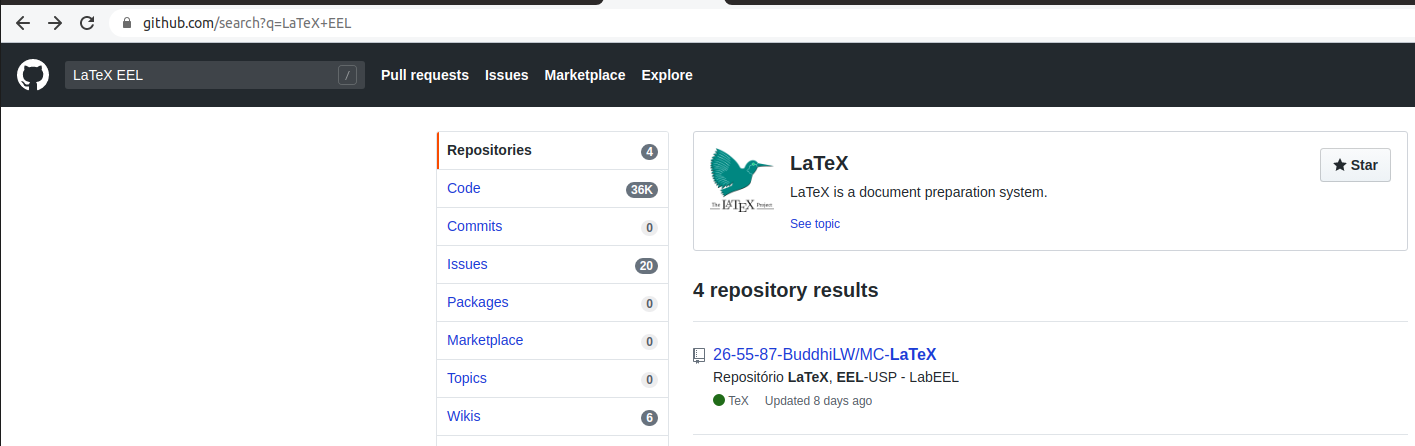
\includegraphics[scale=0.2]{../Imagens/MC1.png}

  \pause

  \begin{tcolorbox}[width=4.5cm, height=6.7mm, top=0.2mm, sharp corners=downhill ]
    Baixar, o repositório:
  \end{tcolorbox}
  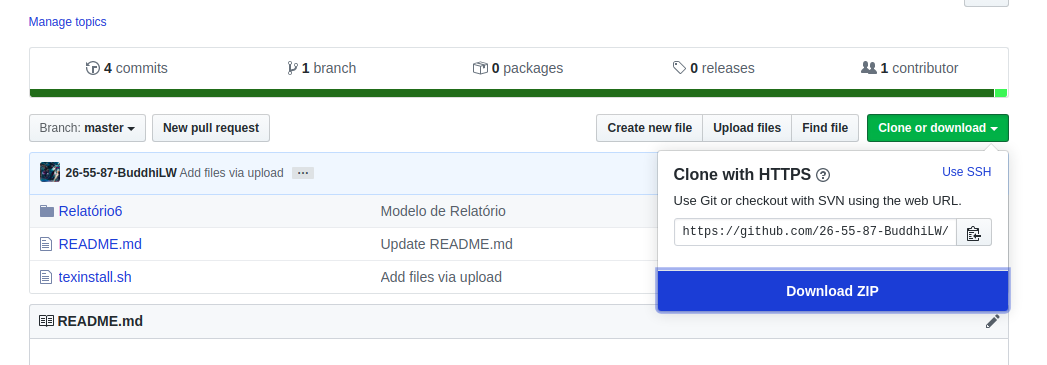
\includegraphics[scale=0.2]{../Imagens/MC3.png}

\end{frame}

\begin{frame}
  \frametitle{Instalação em Linux ou Unix}

  \begin{tcolorbox}[width=12cm, height=10.1mm, top=0.1mm]
    Acessar o diretório com os arquivos baixados, descompactados. E,
    abrir o terminal, no diretório.
  \end{tcolorbox}

  \begin{center}
    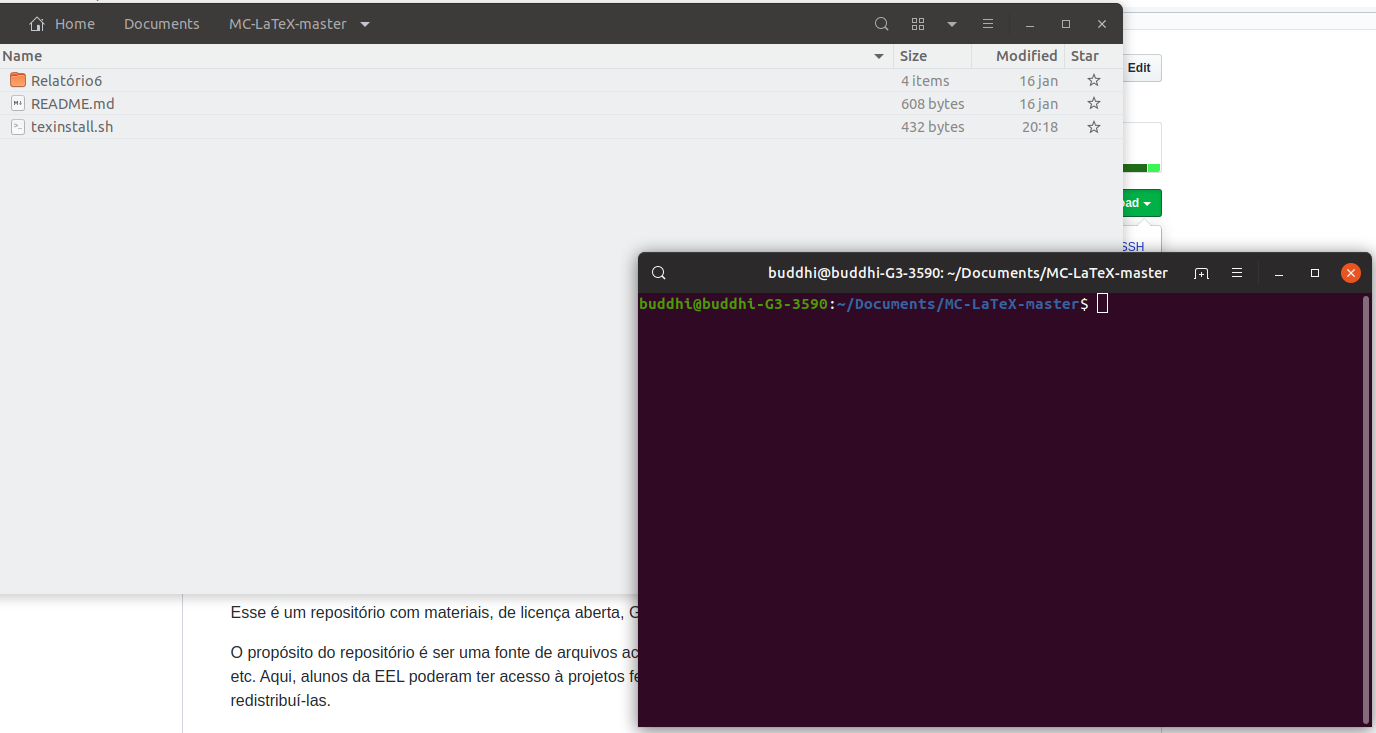
\includegraphics[scale=0.15]{../Imagens/MC4.png}
  \end{center}

  \pause

  \begin{tcolorbox}[sharp corners, width=12cm, height=6.7mm, top=0.2mm]
    Executar o script `'sudo ./texinstall.sh':
  \end{tcolorbox}

  \begin{center}
    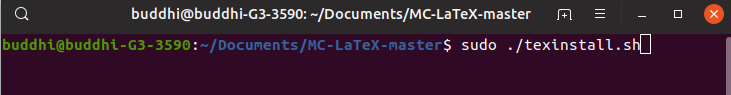
\includegraphics[scale=0.4]{../Imagens/MC5.png}
  \end{center}

\end{frame}


\begin{frame}
  \frametitle{Instalação em Linux ou Unix}
  \begin{tcolorbox}[sharp corners, shadow={2mm}{-1mm}{0mm}{black!50!white}]
    Ou, após, descompactar o arquivo, comande 'sudo chmod +x [diretório
    arquivo.sh]'. E, por fim, comande '[diretório do arquivo]'
  \end{tcolorbox}
  \begin{center}
    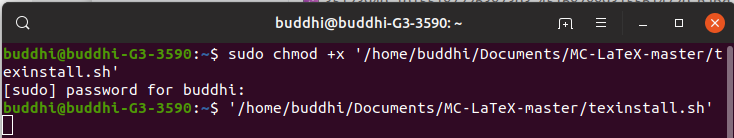
\includegraphics[scale=0.4]{../Imagens/MC6.png}
  \end{center}

  É possível escrever o diretório do arquivo, simplesmente
  arrastando-o ao terminal.

\end{frame}


\begin{frame}

  \section{Instalação em Windows}

  \frametitle{Instalação em Windows, MikTex e TeXstudio}

  \begin{tcolorbox}[fontupper=\fontsize{3.7mm}{3.7mm}, size=small, sharp corners]
    Acesse o site 'texstudio.org', click em Downloads,
  \end{tcolorbox}

  \begin{center}
    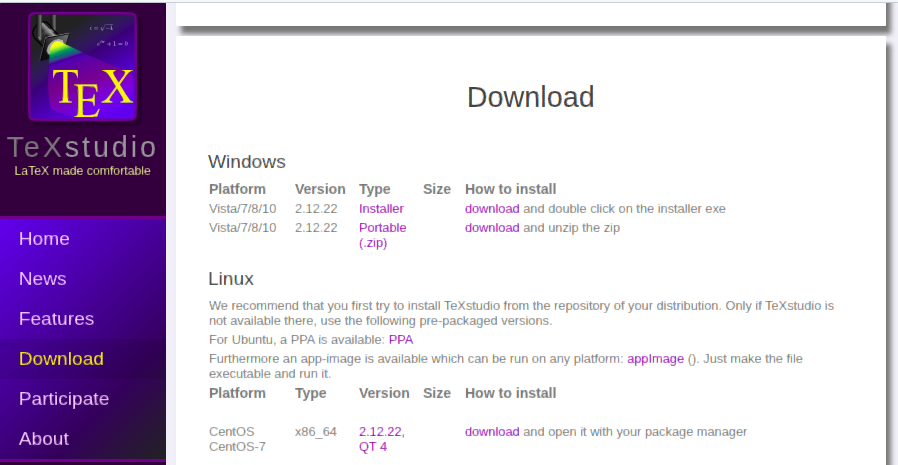
\includegraphics[scale=0.16]{../Imagens/W1.png}
  \end{center}

  \pause

  \begin{tcolorbox}[fontupper=\fontsize{3.5mm}{3.5mm}, size=small, sharp corners]
    Igualmente, acesse o site 'miktex.org/download',
  \end{tcolorbox}

  \begin{center}
    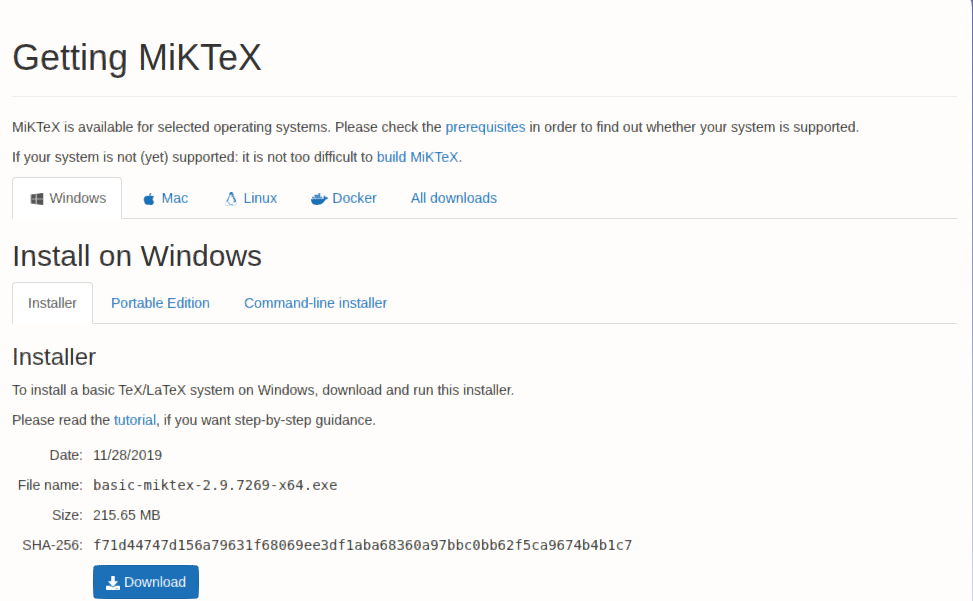
\includegraphics[scale=0.16]{../Imagens/W2.png}
  \end{center}

\end{frame}



\begin{frame}

  \section{TeXstudio, funcionalidades}
  \frametitle{Ambiente de Programação, TeXstudio}
  Acesse, no seu computador, o TeXstudio,
  \begin{center}
    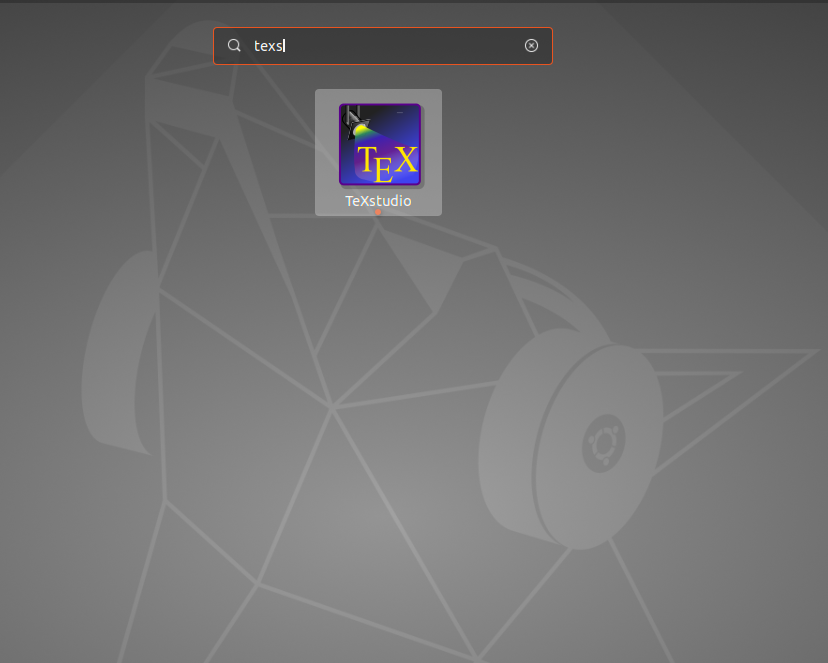
\includegraphics[scale=0.10]{../Imagens/Am1.png}
  \end{center}

  \pause

  \begin{center}
    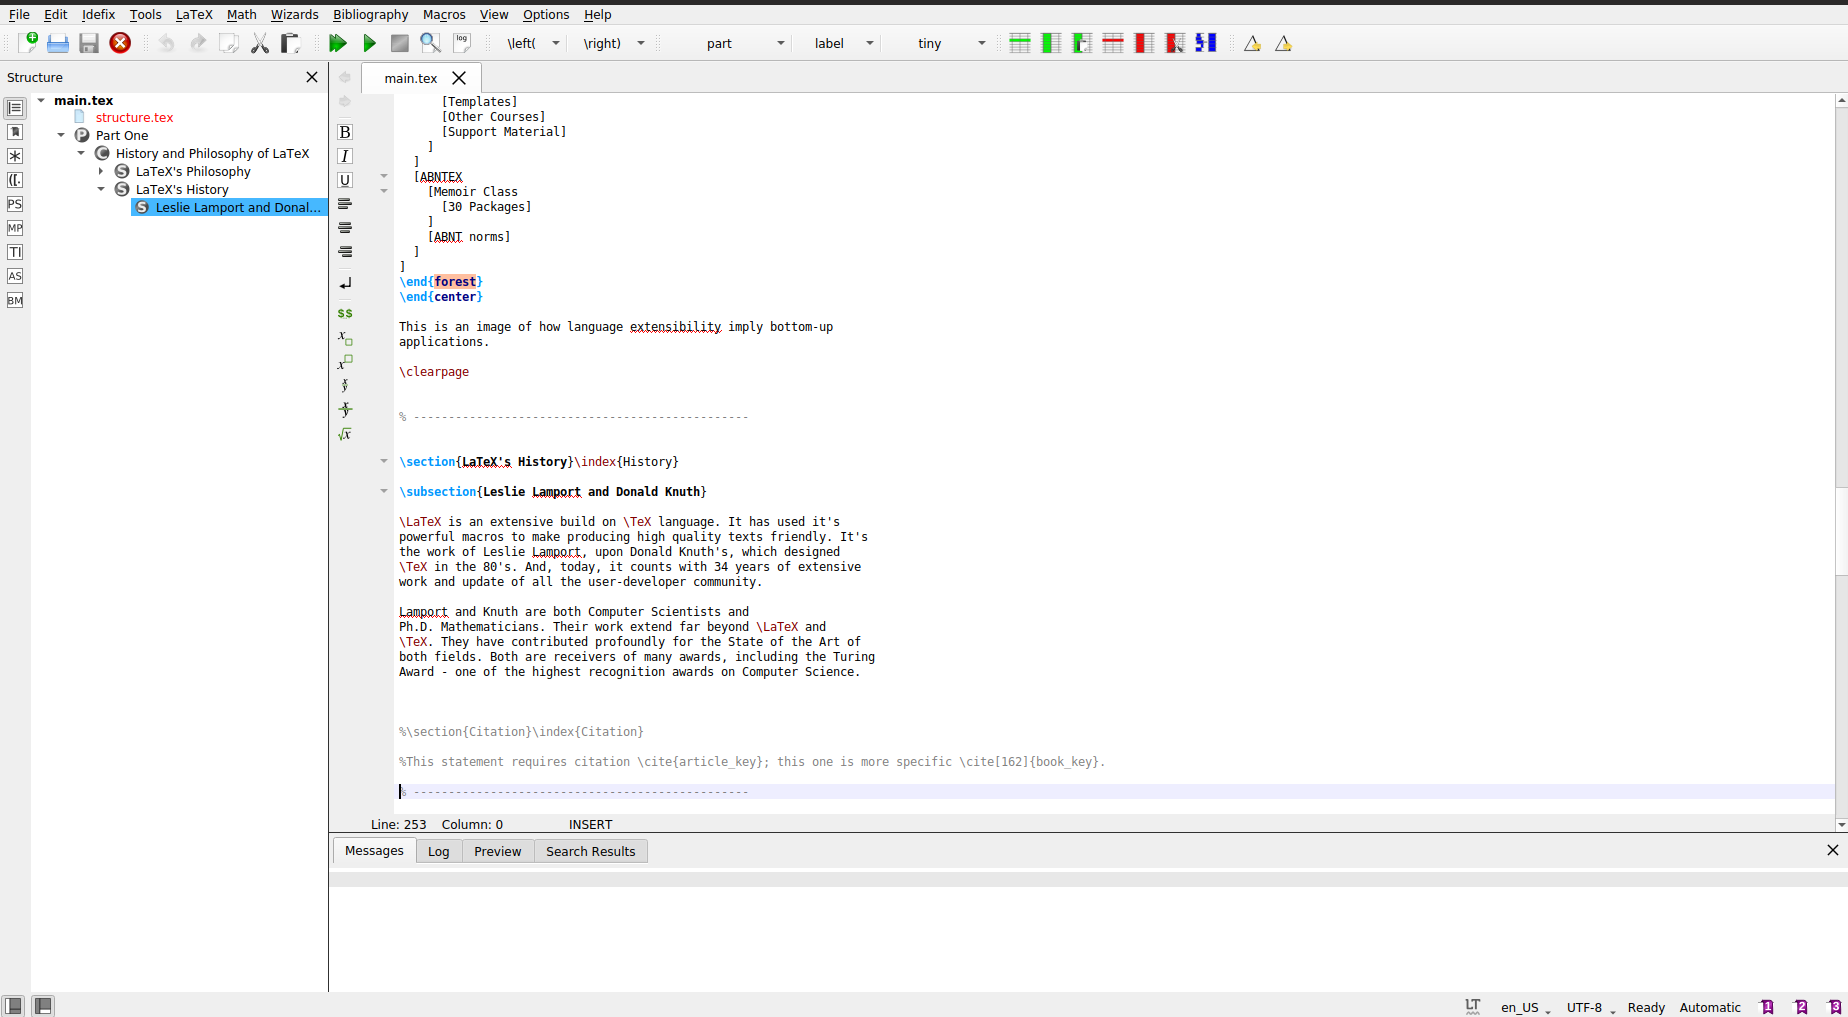
\includegraphics[scale=0.13]{../Imagens/Am2.png}
  \end{center}


\end{frame}

\begin{frame}

  \frametitle{Autocomplete}
  \begin{tcolorbox}[fontupper=\fontsize{5mm}{5mm}, size=small, sharp corners]
  Uma das ferramentas mais importante no TeXstudio, e ambientes de
  programação é o 'Autocomplete',
  \end{tcolorbox}

  \begin{center}
    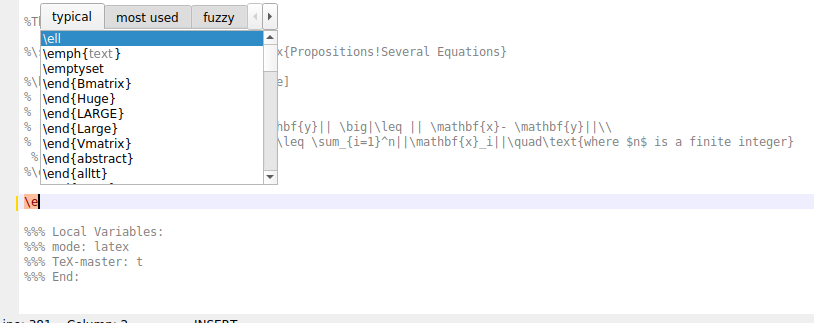
\includegraphics[scale=0.25]{../Imagens/Am3.png}
  \end{center}


  \begin{center}
    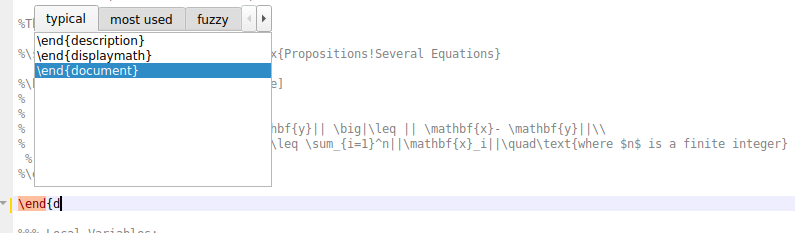
\includegraphics[scale=0.30]{../Imagens/Am4.png}
  \end{center}


\end{frame}



\begin{frame}

  \frametitle{Compilador e Preview}
  \begin{tcolorbox}[fontupper=\fontsize{4mm}{4mm}, size=small, sharp corners]
  É possível Compilar arquivos pressionando 'F6'. E, para ativar o
  Preview, pressionando 'F7'.
  \end{tcolorbox}

  \begin{center}
    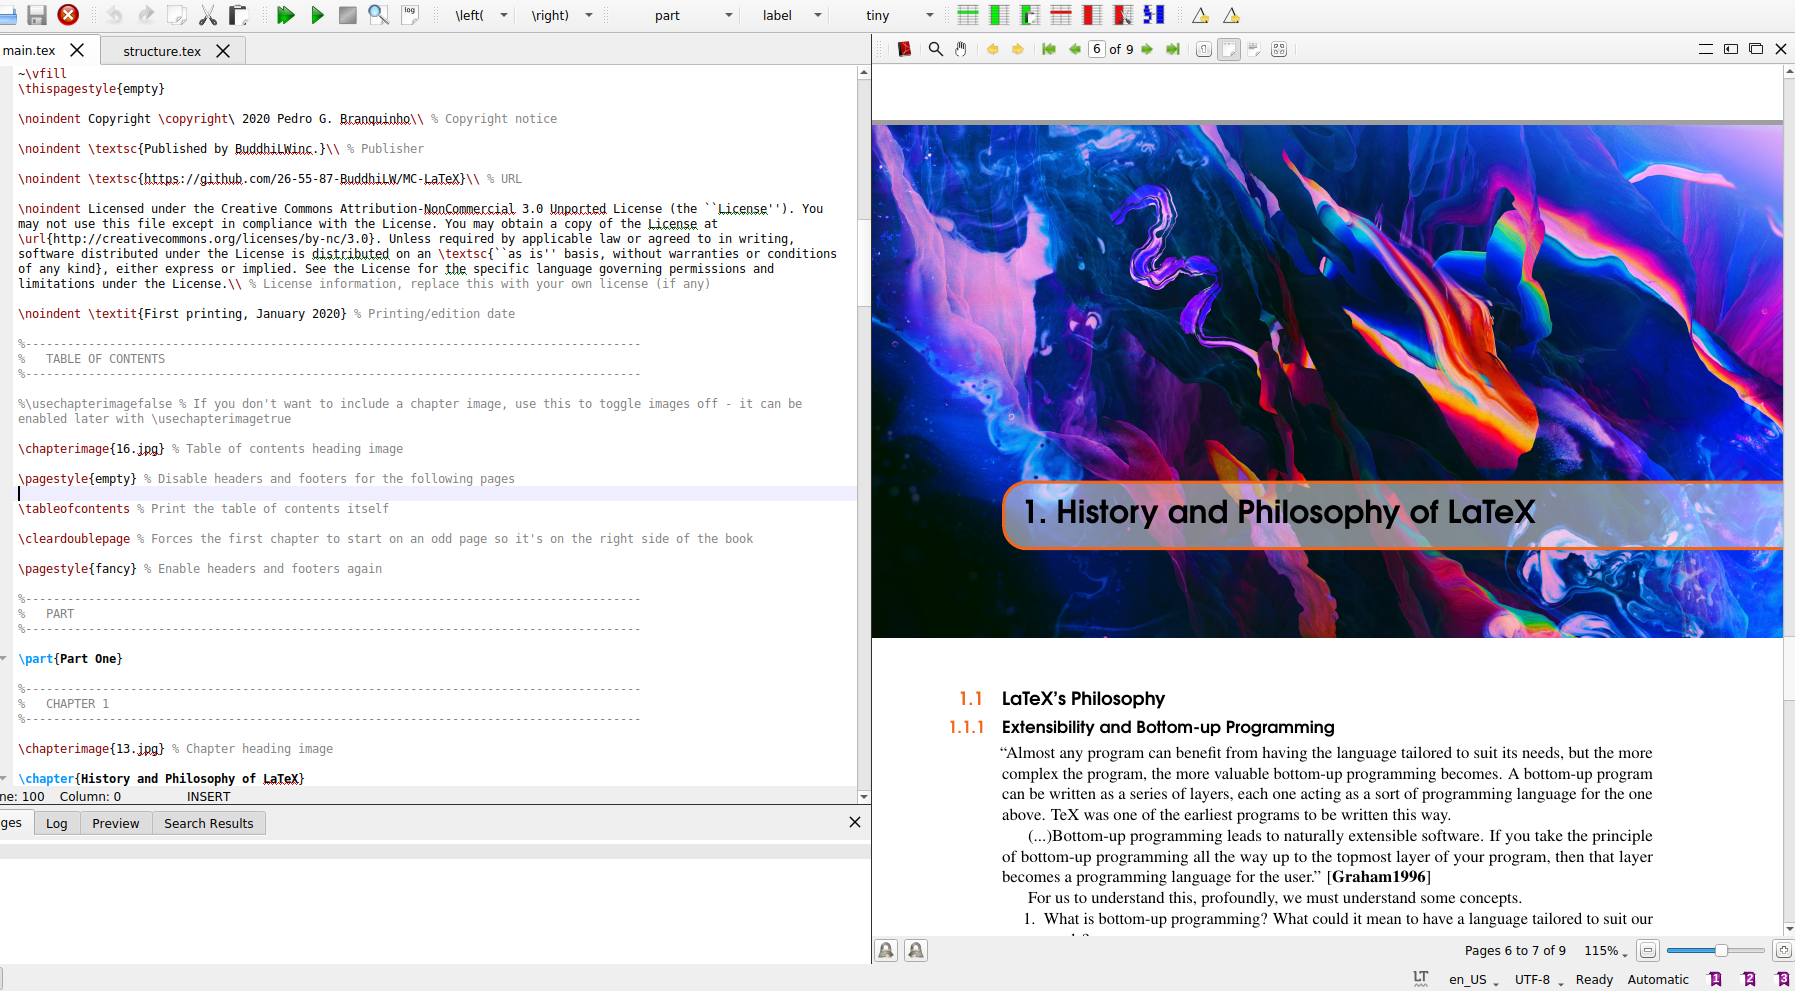
\includegraphics[scale=0.17]{../Imagens/Am6.png}
  \end{center}


\end{frame}


\begin{frame}

  \section{Pacotes, Documentação, e Templates}
  \frametitle{Pacotes e Documentação}
  \begin{tcolorbox}[fontupper=\fontsize{4mm}{4mm}, size=small, sharp
    corners=downhill, colback=red!5!white,colframe=red!75!black]
  Um site fundamental, para o aprofundamento do conhecimento de
  pacotes específicos, utilizados em um
  template é o ctan.org. CTAN é a sigla para Comprehensive TEX Archive
  Network.
  \end{tcolorbox}
  \begin{center}
    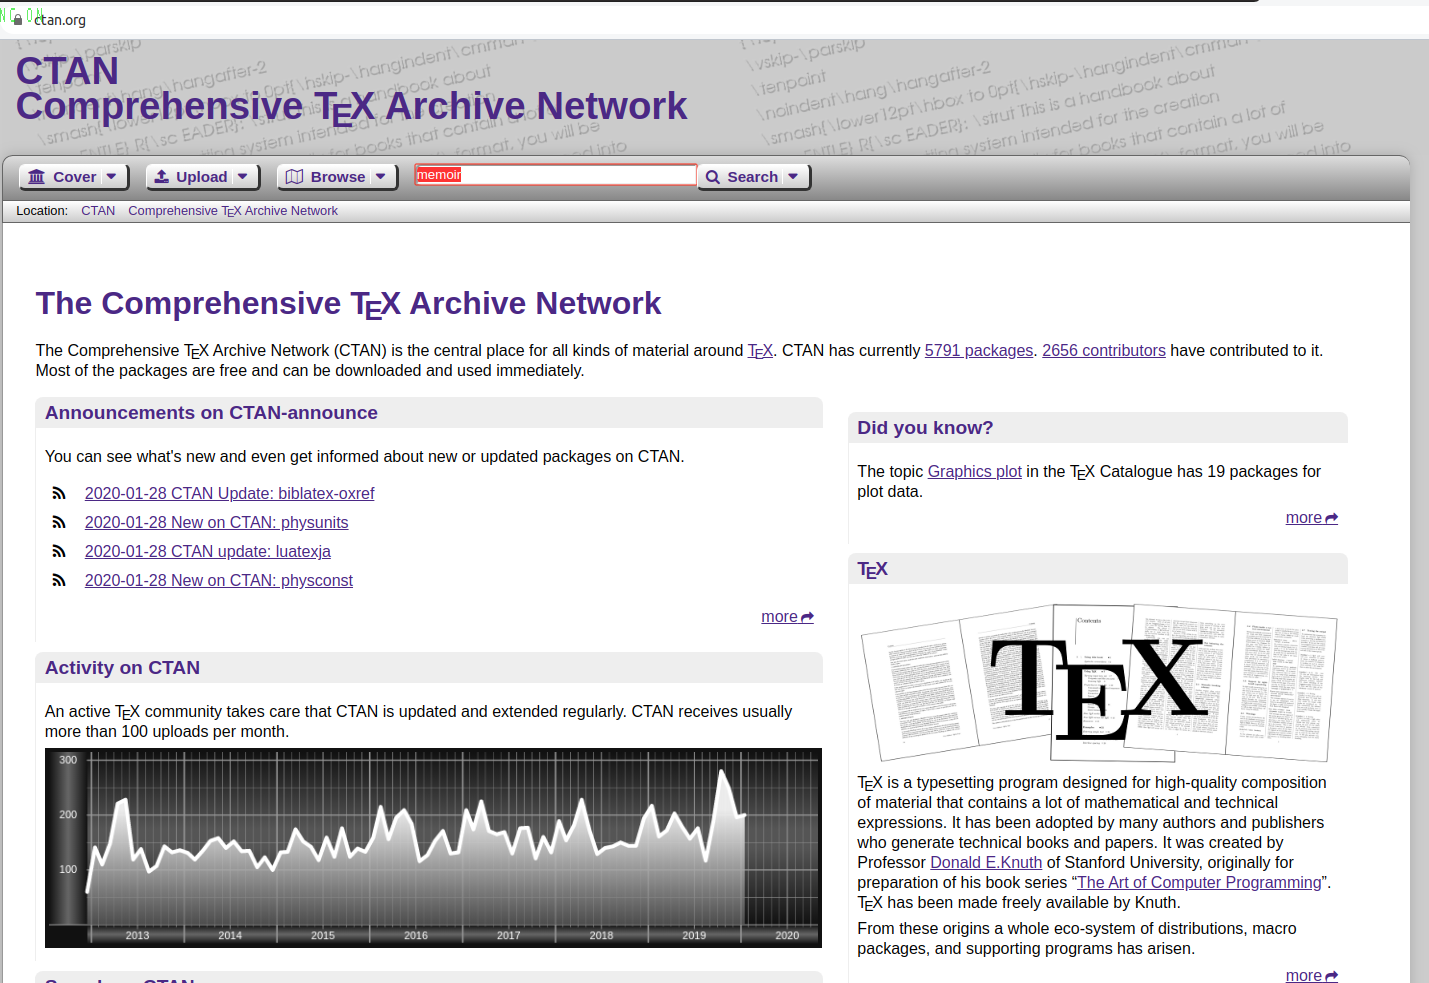
\includegraphics[scale=0.16]{../Imagens/CTAN2.png}
  \end{center}

\end{frame}



\begin{frame}
  \frametitle{Pacotes e Documentação}
  \begin{tcolorbox}[fontupper=\fontsize{4mm}{4mm}, size=small]
    Exemplo: na página da procura ``memoir'', encontramos fontes de
    documentação do pacote. O manual básico nos explica as minúcias do
    funcionamento do pacote. Assim, podemos dominar o funcionamento da formatação
    um documento.
  \end{tcolorbox}

  \begin{center}
    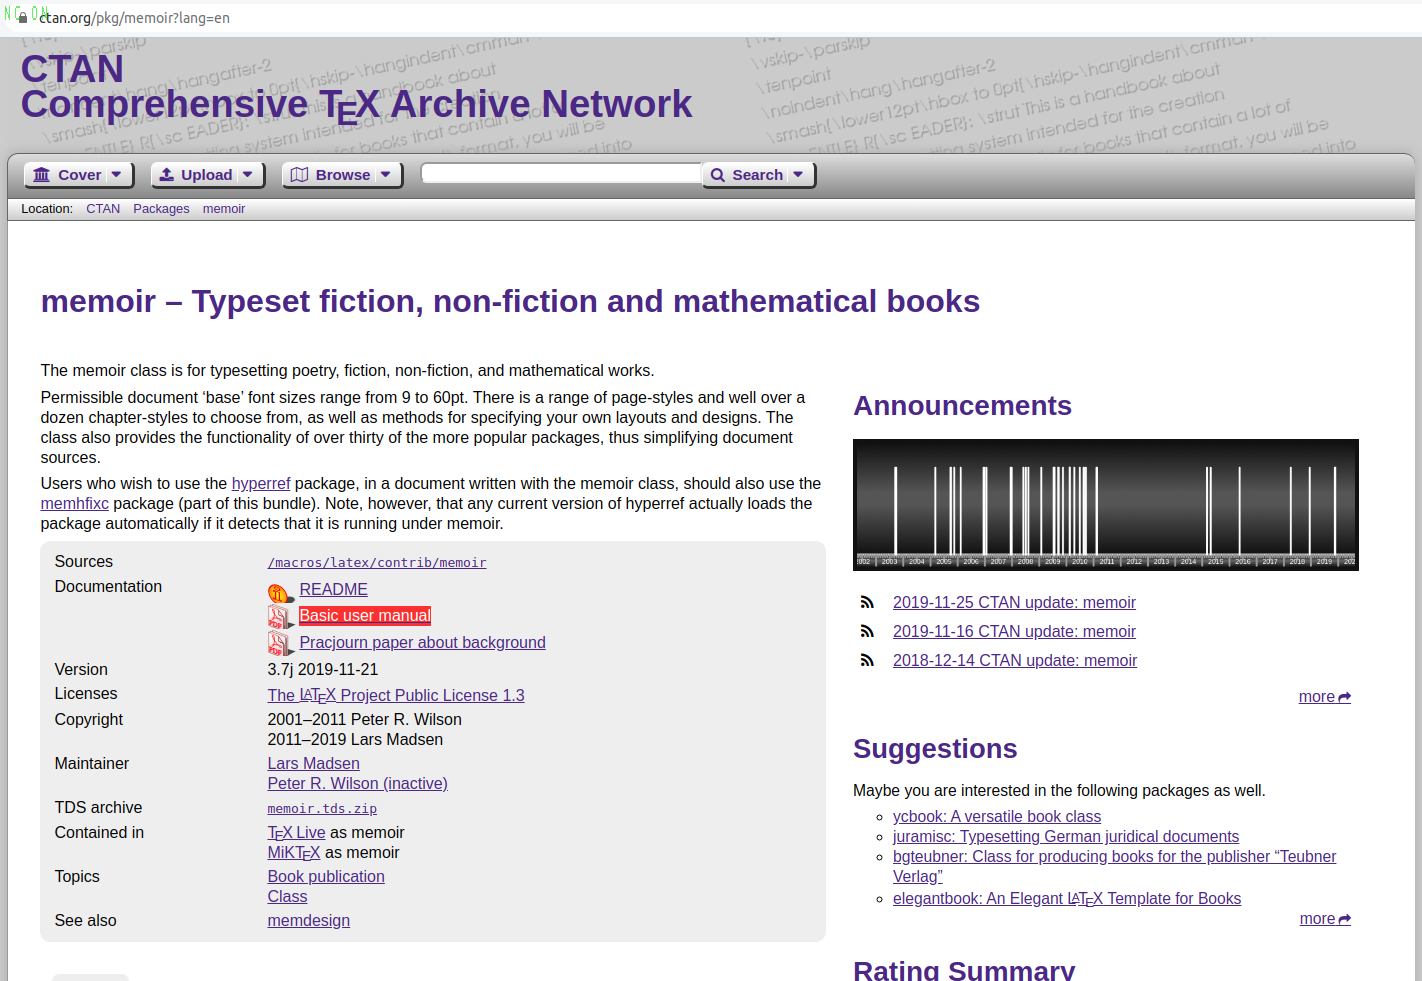
\includegraphics[scale=0.16]{../Imagens/CTAN3.png}
  \end{center}

\end{frame}





\begin{frame}

  \frametitle{Overleaf}
  \begin{tcolorbox}[fontupper=\fontsize{3.7mm}{3.7mm}, size=small]
    Na prática, utilizamos templates parcialmente prontos para nossa
    aplicação. Um site-repositório de templates é ``overleaf.com''.
  \end{tcolorbox}
  \begin{center}
    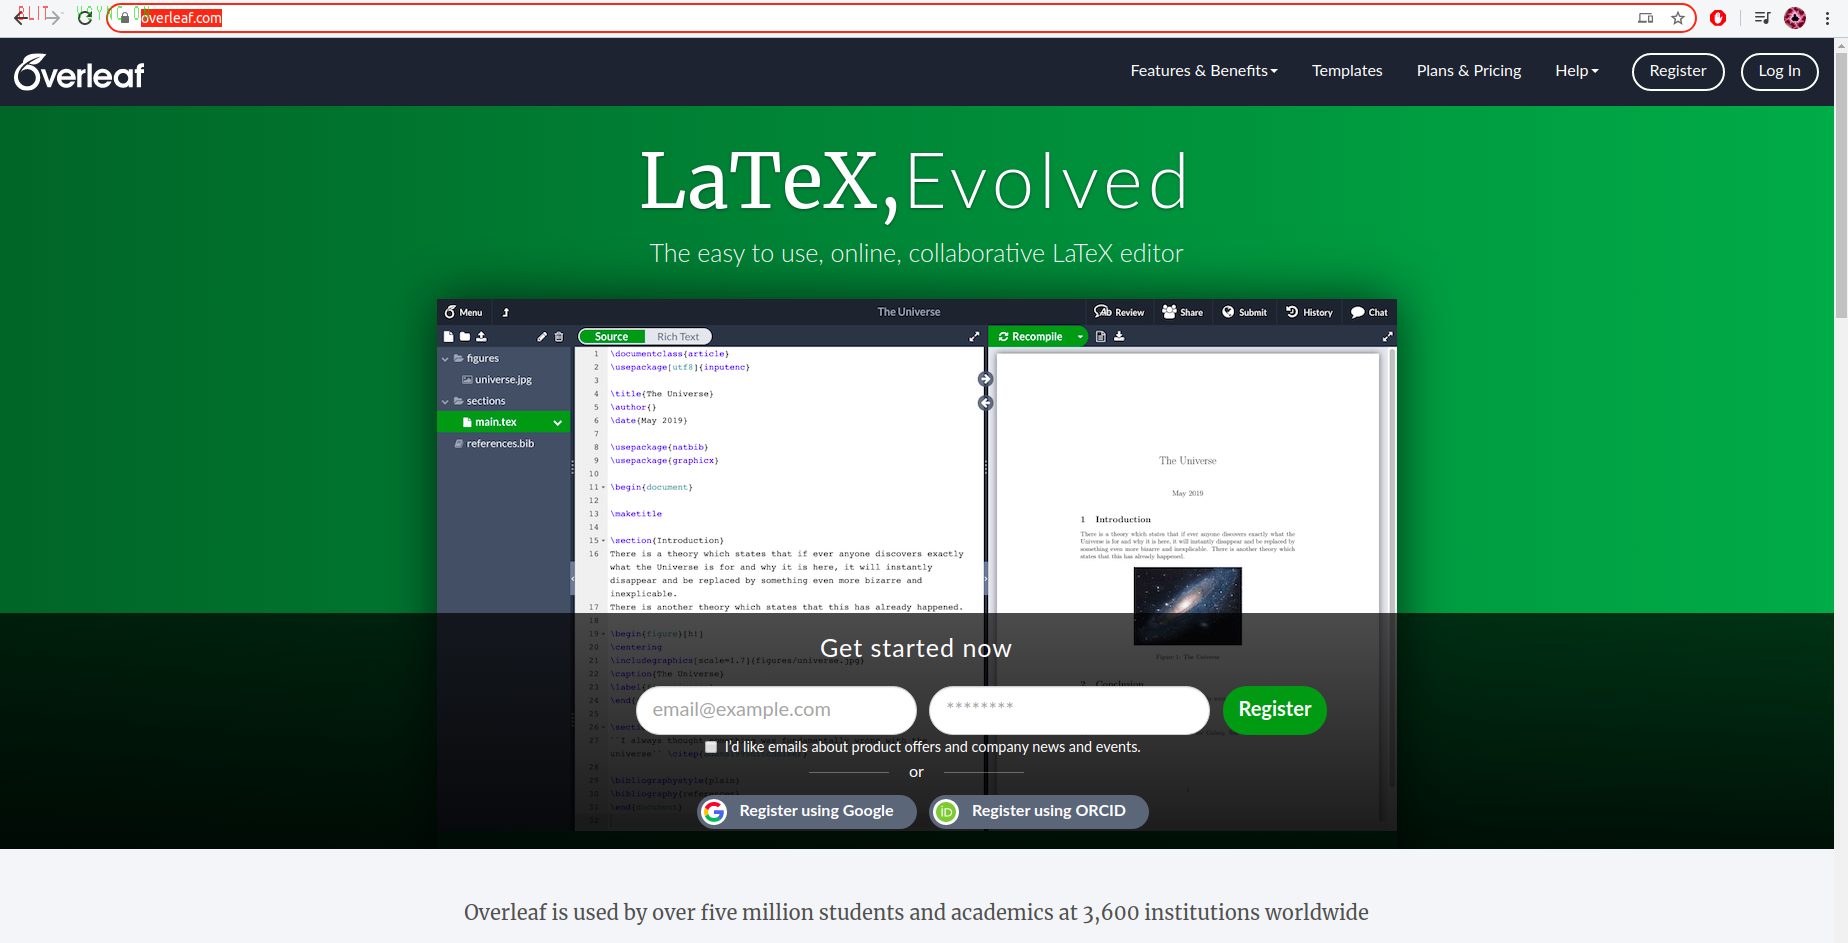
\includegraphics[scale=0.17]{../Imagens/OVERL1.png}
  \end{center}


\end{frame}




\begin{frame}
  \frametitle{Overleaf, Secção Templates}
  Na secção de ``Templates'', encontramos sub-secções de procura,
  particionado pela natureza do trabalho.
  \begin{center}
    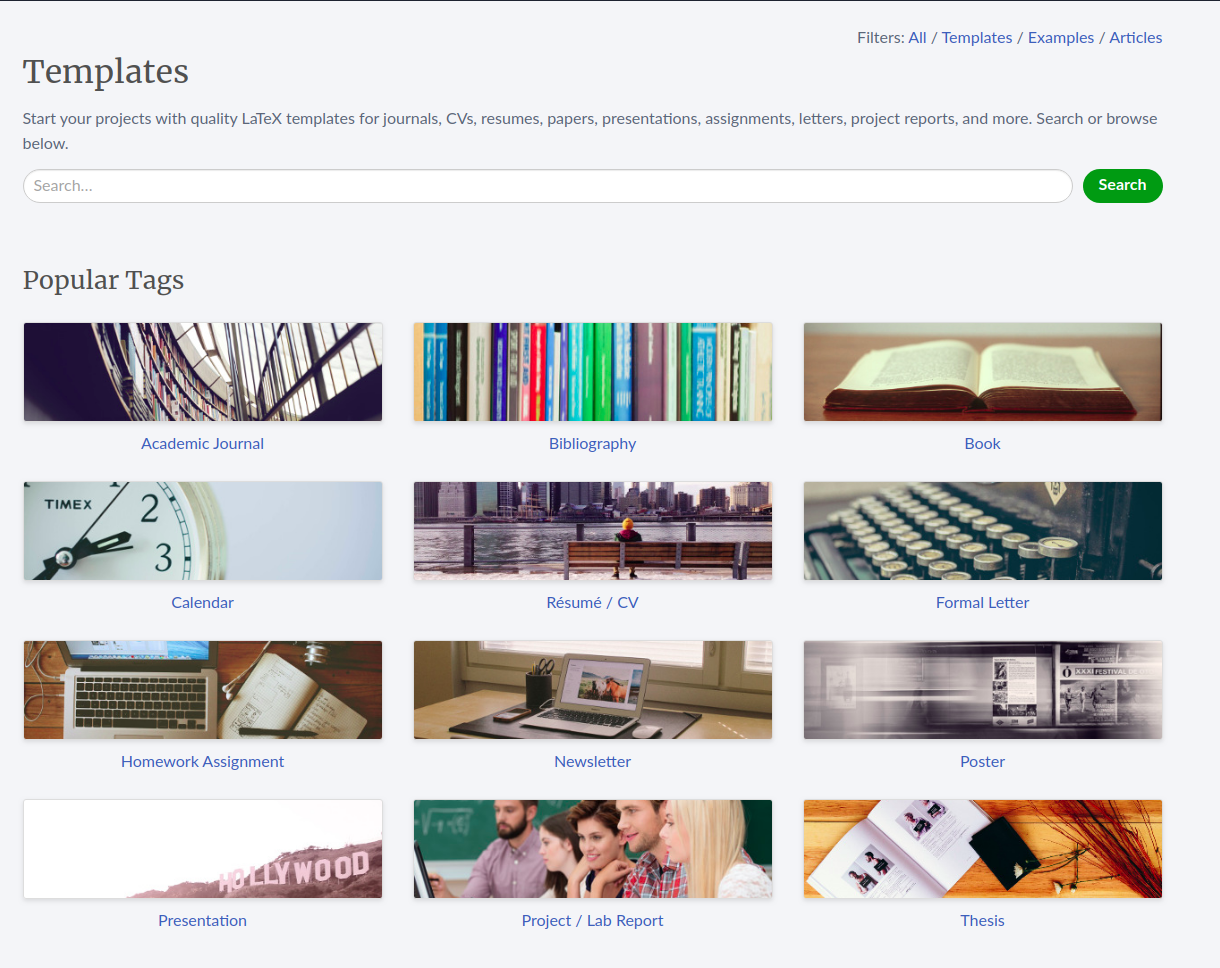
\includegraphics[scale=0.20]{../Imagens/OVERL2.png}
  \end{center}

\end{frame}


\begin{frame}
  \section{Utilização de Template}
  \frametitle{Utilizando Templates da EEL-USP}
  Utilizaremos o arquivo ``Relatório6'', o qual estava dentro do
  conjunto de arquivos baixados, do repositório no GitHub.

  \begin{center}
    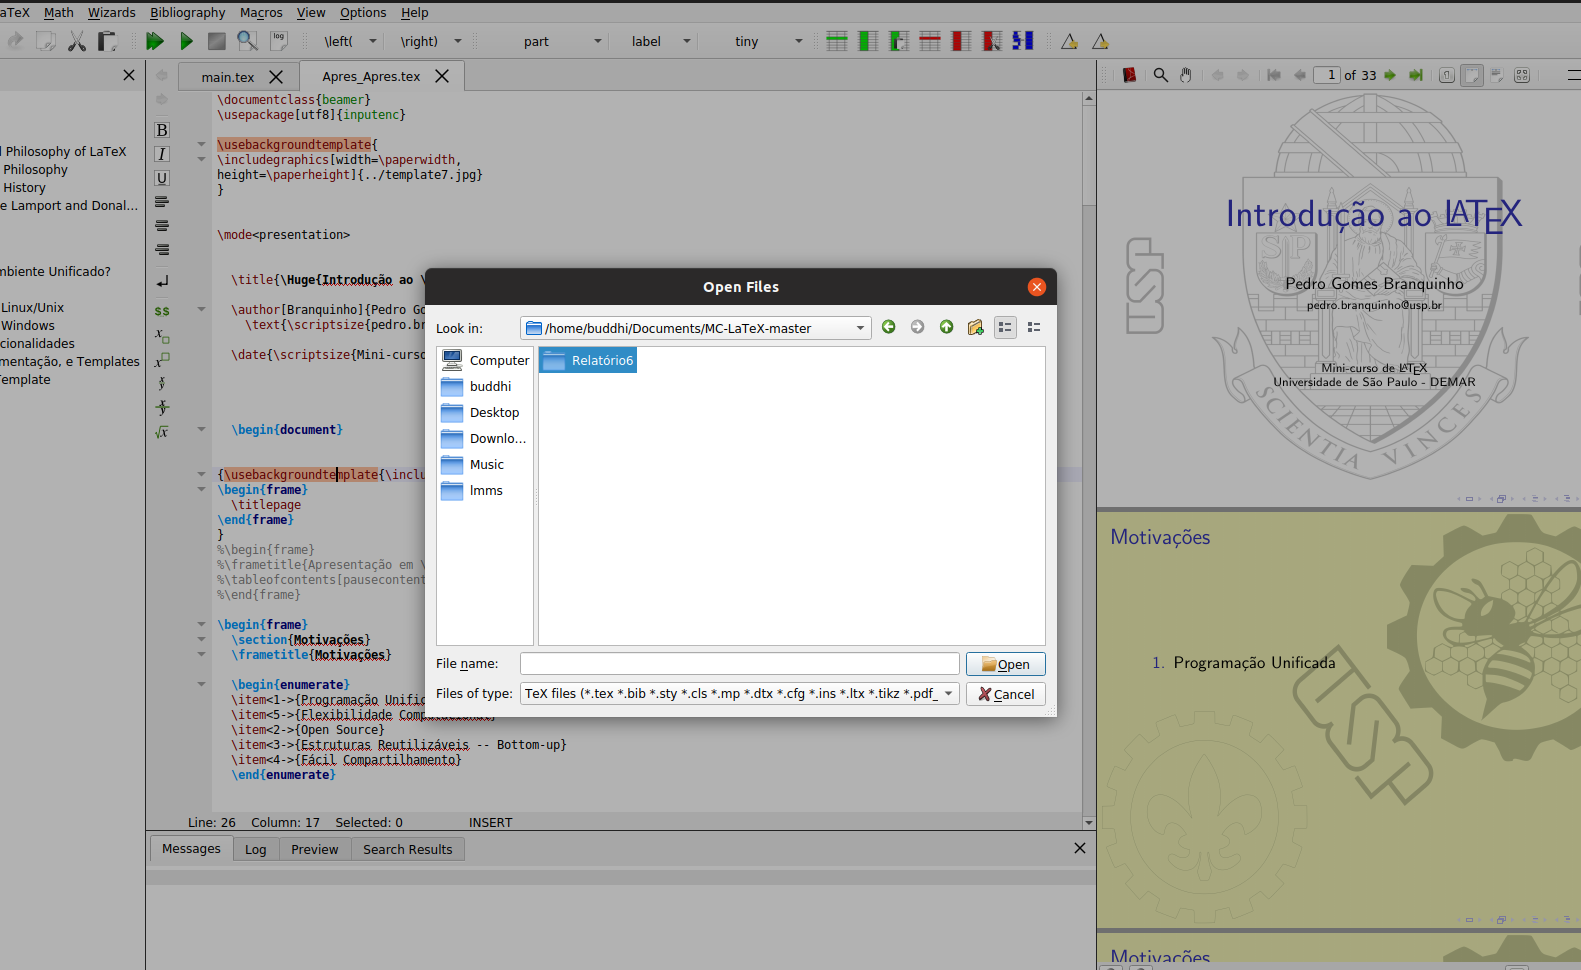
\includegraphics[scale=0.20]{../Imagens/ST1.png}
  \end{center}
\end{frame}



\begin{frame}

  \frametitle{Utilizando Templates da EEL-USP}

  Abrindo o arquivo ``Relatório6/Relatório6.tex'' dentro do TeXstudio,
  Compile (F6) e Visualize (F7).

  \begin{center}
    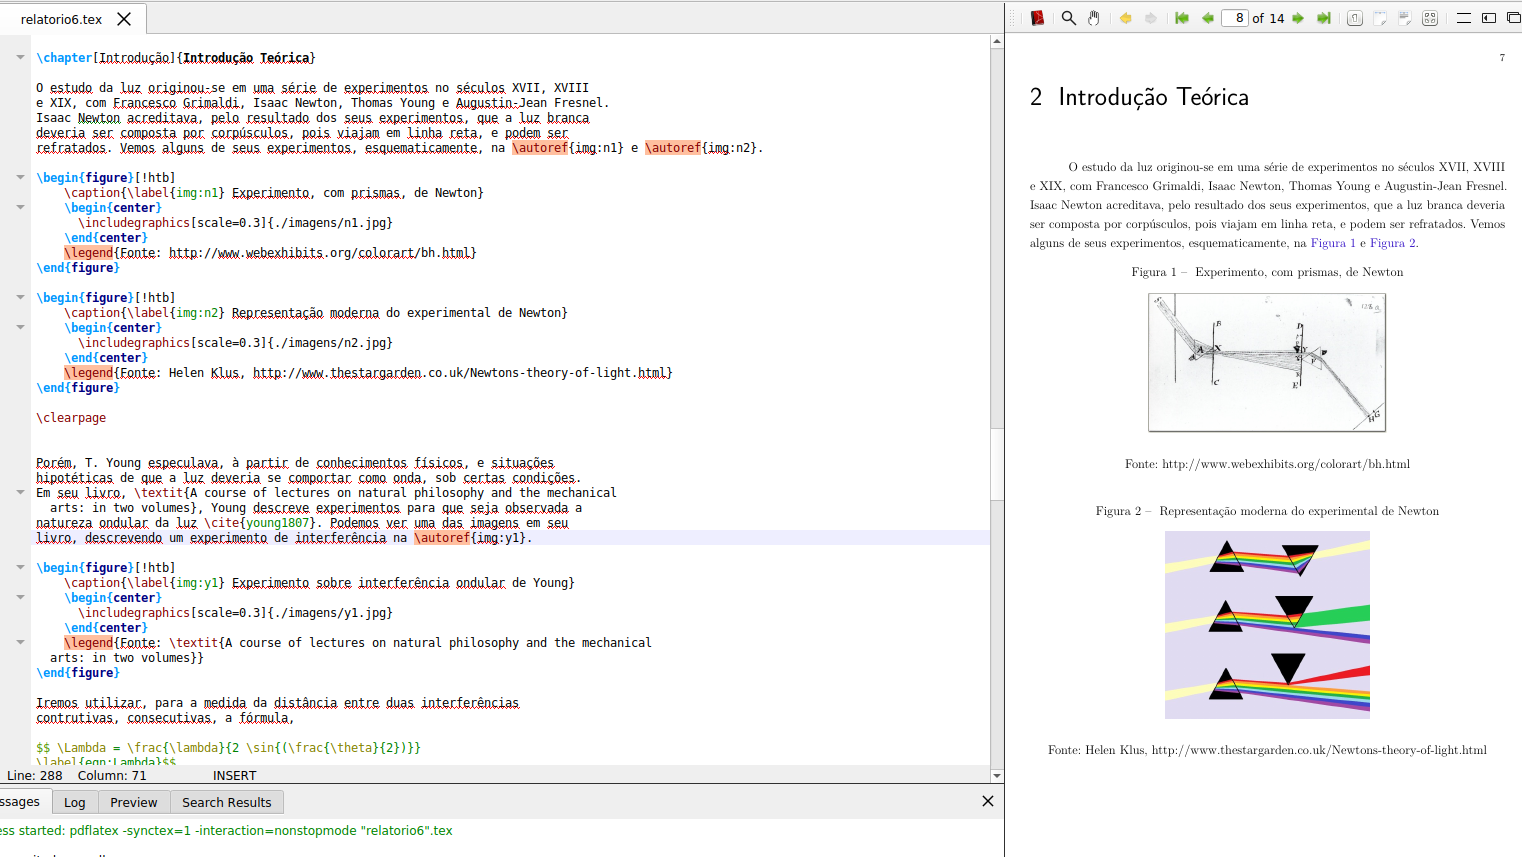
\includegraphics[scale=0.20] {../Imagens/ST3.png}
  \end{center}


\end{frame}





\begin{frame}

  \section{Exercícios}
  \frametitle{Em casa, faça os exercícios do capítulo 1}

  Os exercícios consistem em manipular parâmetros do template do
  relatório. Alguns deles são, por exemplo, a fonte, e tamanho.

  \begin{center}
    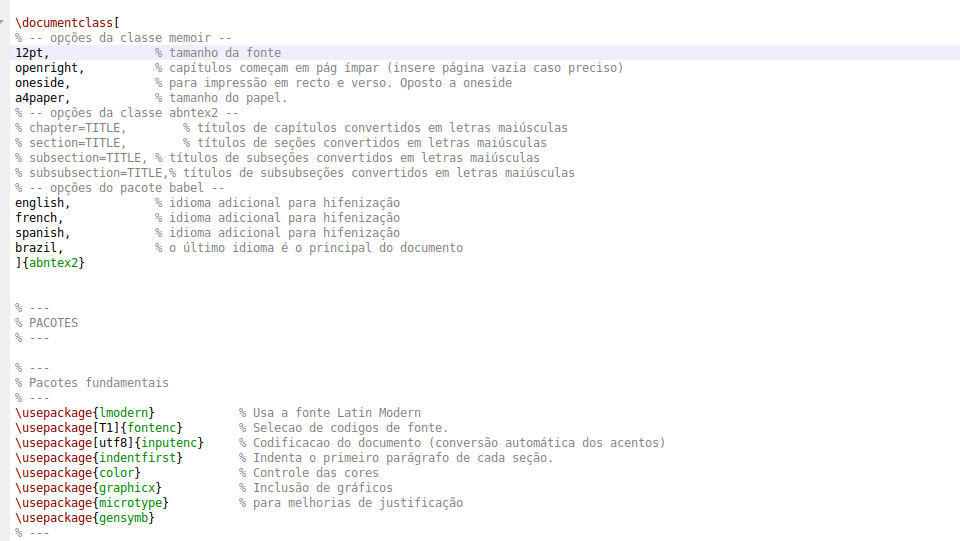
\includegraphics[scale=0.30] {../Imagens/ST4.png}
  \end{center}

\end{frame}

\begin{frame}

  \frametitle{Em casa, faça os exercícios do capítulo 1}

  Espaçamento de linha e parágrafo.

  \begin{center}
    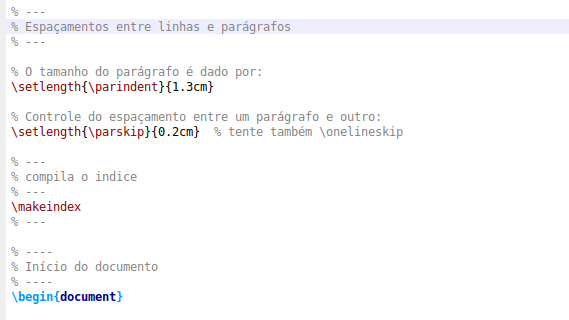
\includegraphics[scale=0.40] {../Imagens/ST5.png}
  \end{center}


\end{frame}

\end{document}

%%% Local Variables:
%%% mode: latex
%%% TeX-master: t
%%% End:


%%%%%%%%%% DIFF PREAMBULO

%% Definindo minha(s) cor(es) para os blocos
% \mdfdefinestyle{ver1}{%
%   linecolor=red!40!black,outerlinewidth=1pt,%
%   frametitlerule=true,frametitlefont=\sffamily\bfseries\color{white},%
%   frametitlerulewidth=1pt,frametitlerulecolor=red!10!black,%
%   frametitlebackgroundcolor=red!20!black,
%   backgroundcolor=red!5,
%   innertopmargin=\topskip,
%   roundcorner=5pt
% }

% \mdfdefinestyle{ver2}{%
%   linecolor=green!40!black,outerlinewidth=1pt,%
%   frametitlerule=true,frametitlefont=\sffamily\bfseries\color{white},%
%   frametitlerulewidth=1pt,frametitlerulecolor=green!40!black,%
%   frametitlebackgroundcolor=green!40!black,
%   backgroundcolor=green!5,
%   innertopmargin=\topskip,
%   roundcorner=5pt
% }

% \mdfdefinestyle{viol1}{%
%   linecolor=green!40!black,outerlinewidth=1pt,%
%   frametitlerule=true,frametitlefont=\sffamily\bfseries\color{white},%
%   frametitlerulewidth=1pt,frametitlerulecolor=green!40!black,%
%   frametitlebackgroundcolor=green!40!black,
%   backgroundcolor=green!5,
%   innertopmargin=\topskip,
%   roundcorner=5pt
% }

% %% Definindo o am.ver.1(ambiente vermelho 1), com o stilo (style=mystyle),
% %% 'exa' é um variável arbitrário. Isto é, não será utilizada explicitamente.
% \newmdenv[style=ver1]{exa1}
% \newenvironment{amver1}[1]
% {\begin{exa1}[frametitle=#1]}
%   {\end{exa1}}

% %% am. ver. 2
% \newmdenv[style=ver2]{exa2}
% \newenvironment{amver2}[1]
% {\begin{exa2}[frametitle=#1]}
%   {\end{exa2}}

% %% am. viol. 1
% \newmdenv[style=viol1]{exa3}
% \newenvironment{amviol1}[1]
% {\begin{exa3}[frametitle=#1]}
%   {\end{exa3}}
